\documentclass[11pt]{article}
\usepackage[margin=1in]{geometry}
\usepackage{amsmath,amssymb}
\usepackage{booktabs}
\usepackage{graphicx}
\usepackage{microtype}
\usepackage{array}
\title{Supplement to Repair What Matters}
\author{Swayam Singal}
\date{}
\begin{document}
\maketitle

\section{What this supplement adds}
The main paper contains the revision contract, the full paper-grade campaign, and the residual-sensitive confirmation. This supplement collects three details that are useful for review but awkward to fit into the main narrative: how calibrated work should be interpreted, representative trained-3DGS decision cases, and the display-space bound used by the residual-sensitive mechanism study.

\section{Calibrated work and practical benefit}
The planner compares a candidate local repair with a frozen full-rebuild baseline using
\[
W(C)=\sum_d \kappa_d n_d(C).
\]
Here $n_d(C)$ is a native counter and $\kappa_d$ is the pre-campaign conversion factor for that counter's domain. The paper-grade campaign calibrates Gaussian inspection, Gaussian update, GPU-publication bytes, and temporal-invalidated pixels. This produces a common work scale without treating those native operations as interchangeable physical events.

A ratio below one means the selected repair accounts for less work than the independently measured full baseline on this frozen scale. A ratio of one denotes \textsc{Full} fallback. The metric deliberately excludes wall-clock effects such as allocator behavior, cache locality, synchronization, command submission, and GPU overlap.

\begin{table}[h]
\centering
\caption{Paper-grade calibrated-work interpretation by dataset/representation. ``Work avoided'' is $1-\mathrm{median}(W/W_{\mathrm{full}})$.}
\begin{tabular}{lrr}
\toprule
Dataset / representation & Median work/\textsc{Full} & Median work avoided \\
\midrule
3RScan & 0.341 & 65.94\% \\
ARKitScenes & 0.483 & 51.68\% \\
Bonn RGB-D Dynamic & 0.475 & 52.45\% \\
Trained GraphDECO 3DGS & 0.519 & 48.09\% \\
Overall & 0.474 & 52.55\% \\
\bottomrule
\end{tabular}
\end{table}

\section{Representative trained-3DGS behavior}
The next figures use a pinned pretrained GraphDECO 3DGS scene from the frozen evaluation. They are revision-fidelity visualizations: the selected repair is compared with a full-after result inside the same representation.

\begin{figure}[h]
\centering
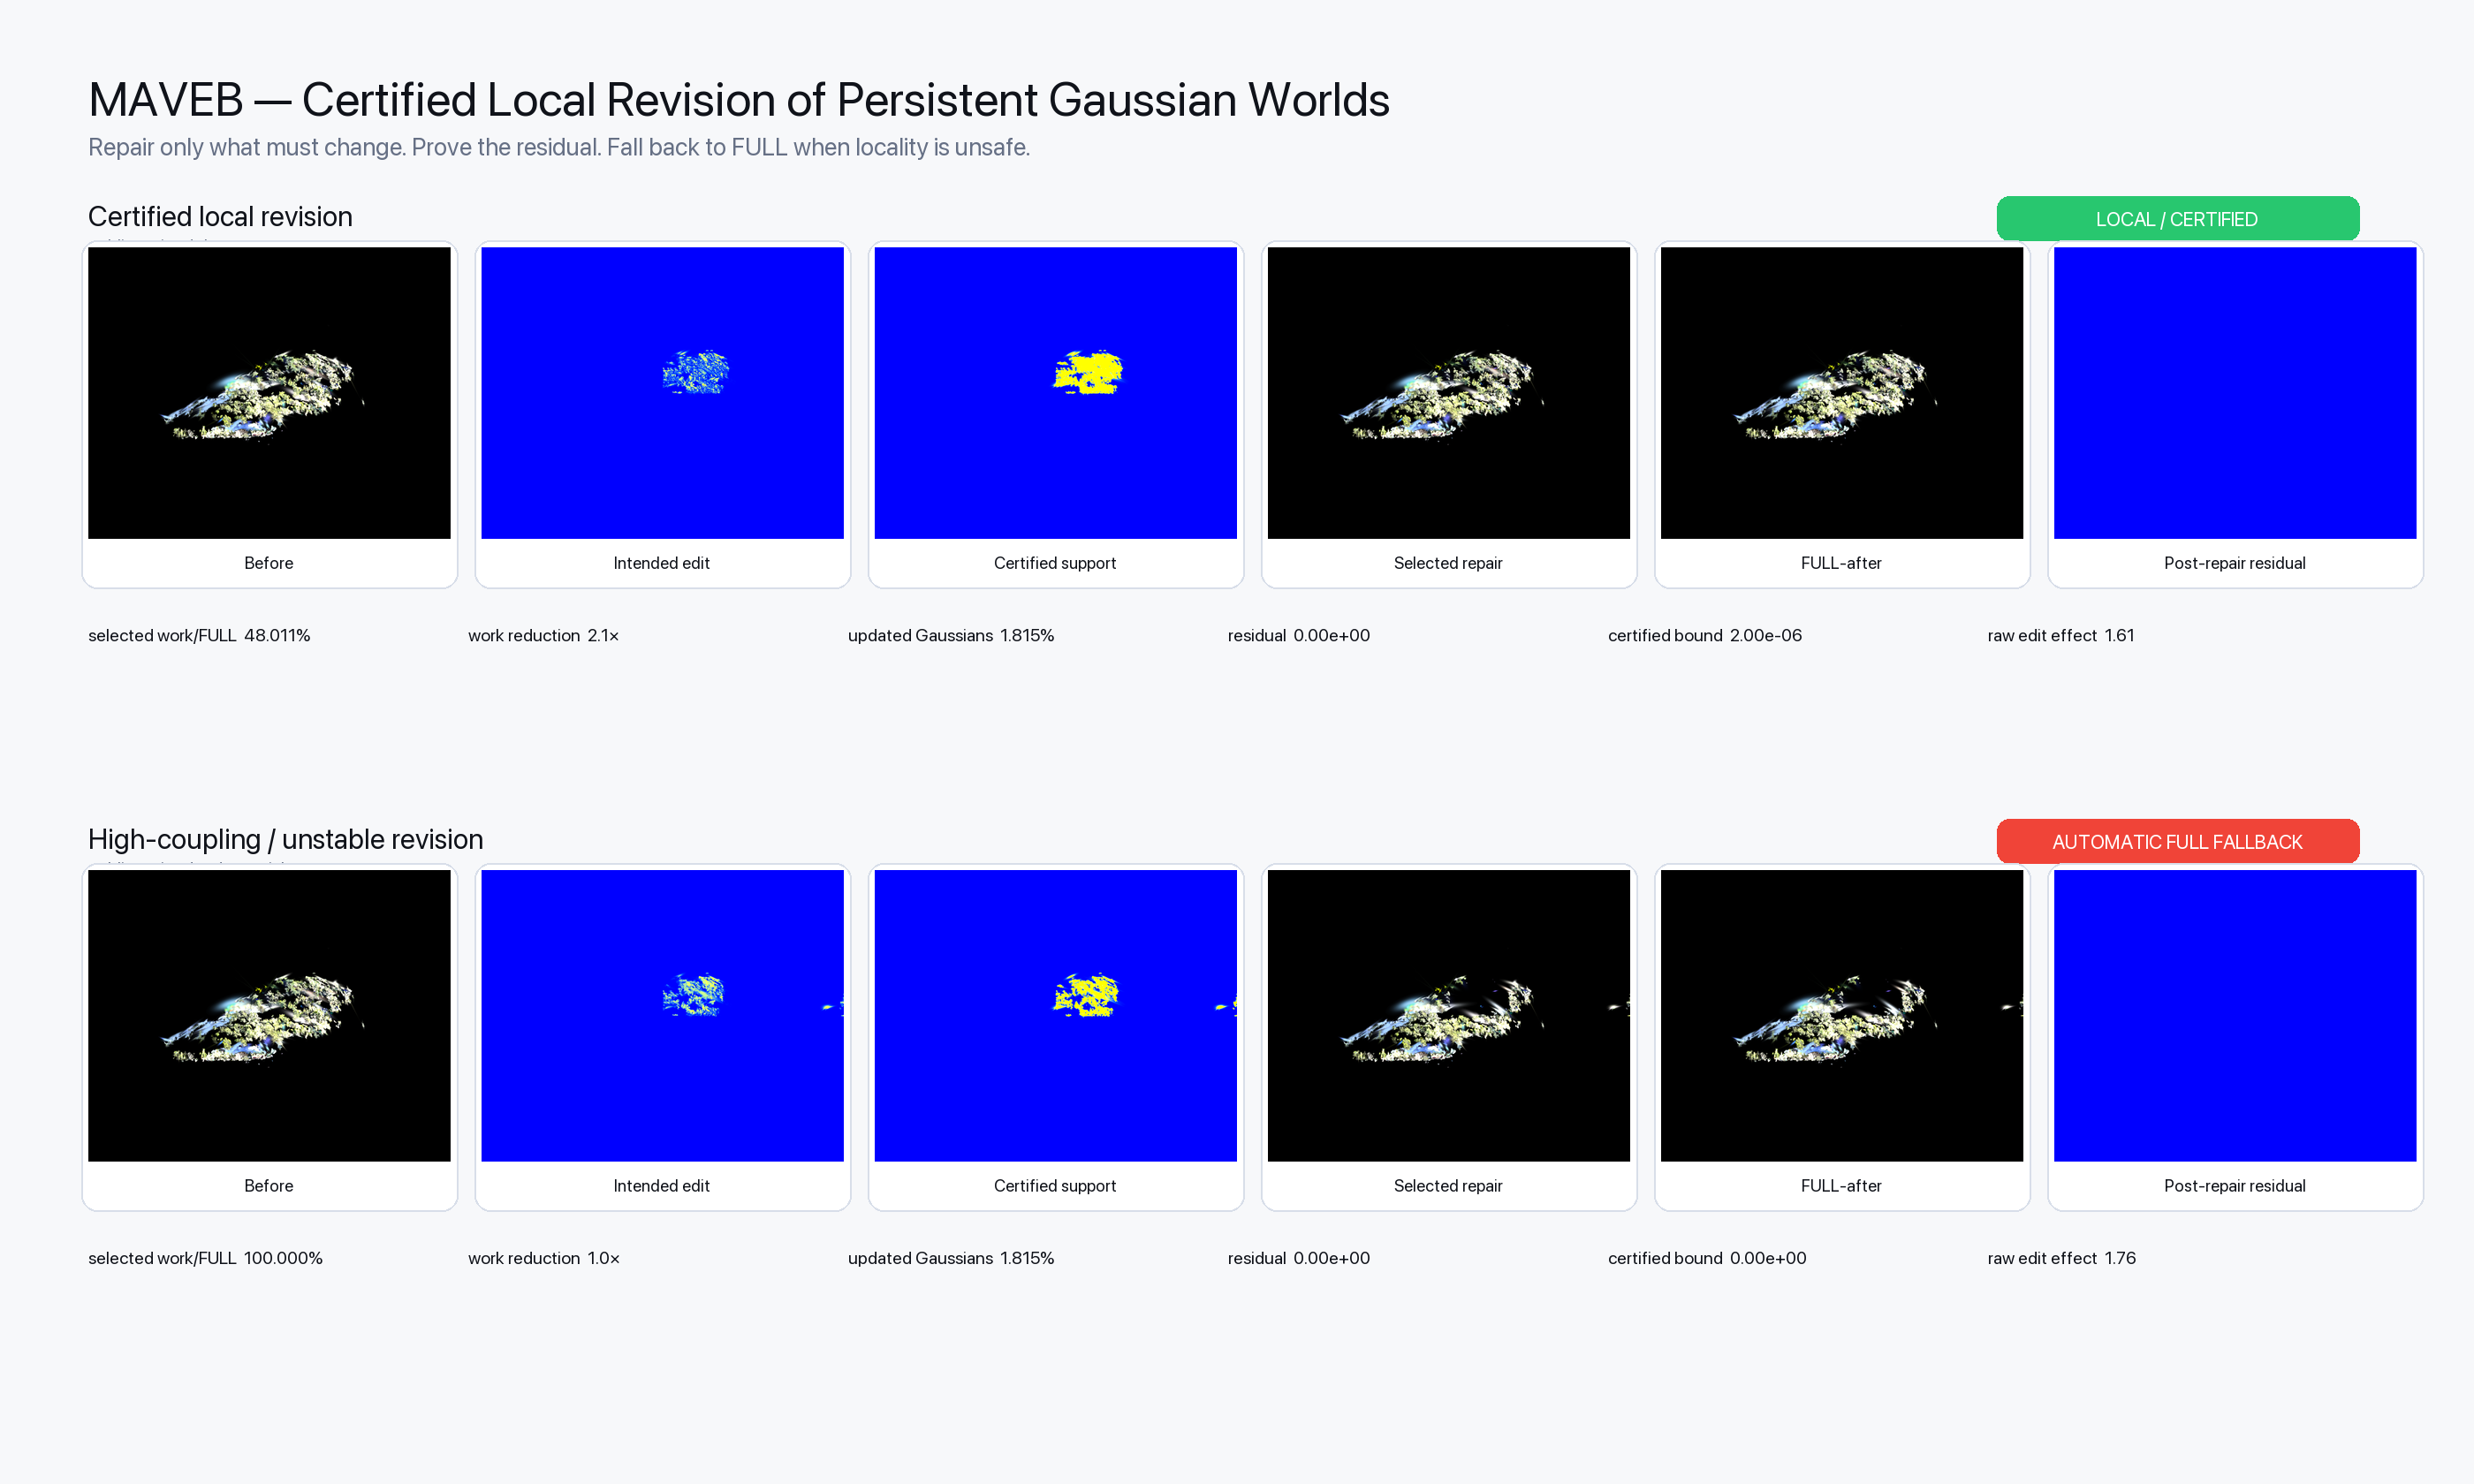
\includegraphics[width=\textwidth]{figures/trained_3dgs_qualitative.png}
\caption{A certified local case and an automatic full fallback on the same trained-3DGS representation. The local case records work/\textsc{Full}=48.011\%; the fallback records 100\%.}
\end{figure}

\begin{figure}[h]
\centering
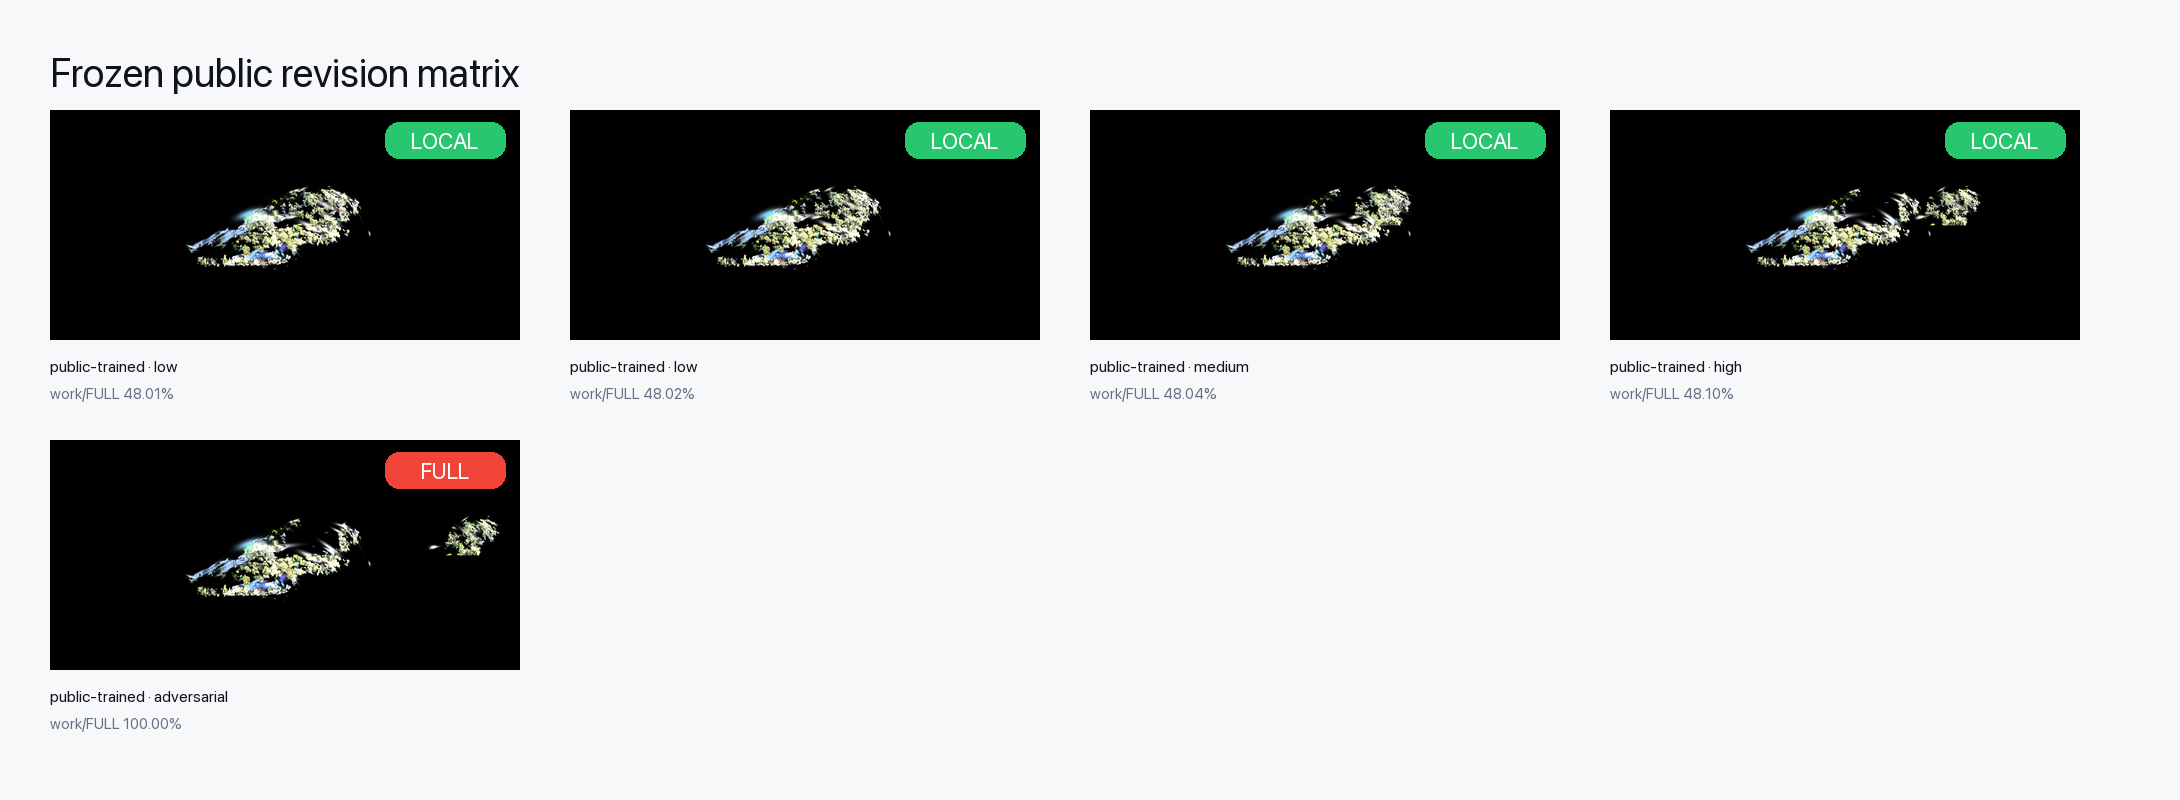
\includegraphics[width=\textwidth]{figures/trained_3dgs_case_mosaic.png}
\caption{Frozen coupling sweep on a trained-3DGS scene. Low, medium, and one high-coupling case remain local at roughly 48\% of the calibrated full baseline, while the adversarial case selects \textsc{Full}.}
\end{figure}

\begin{figure}[h]
\centering
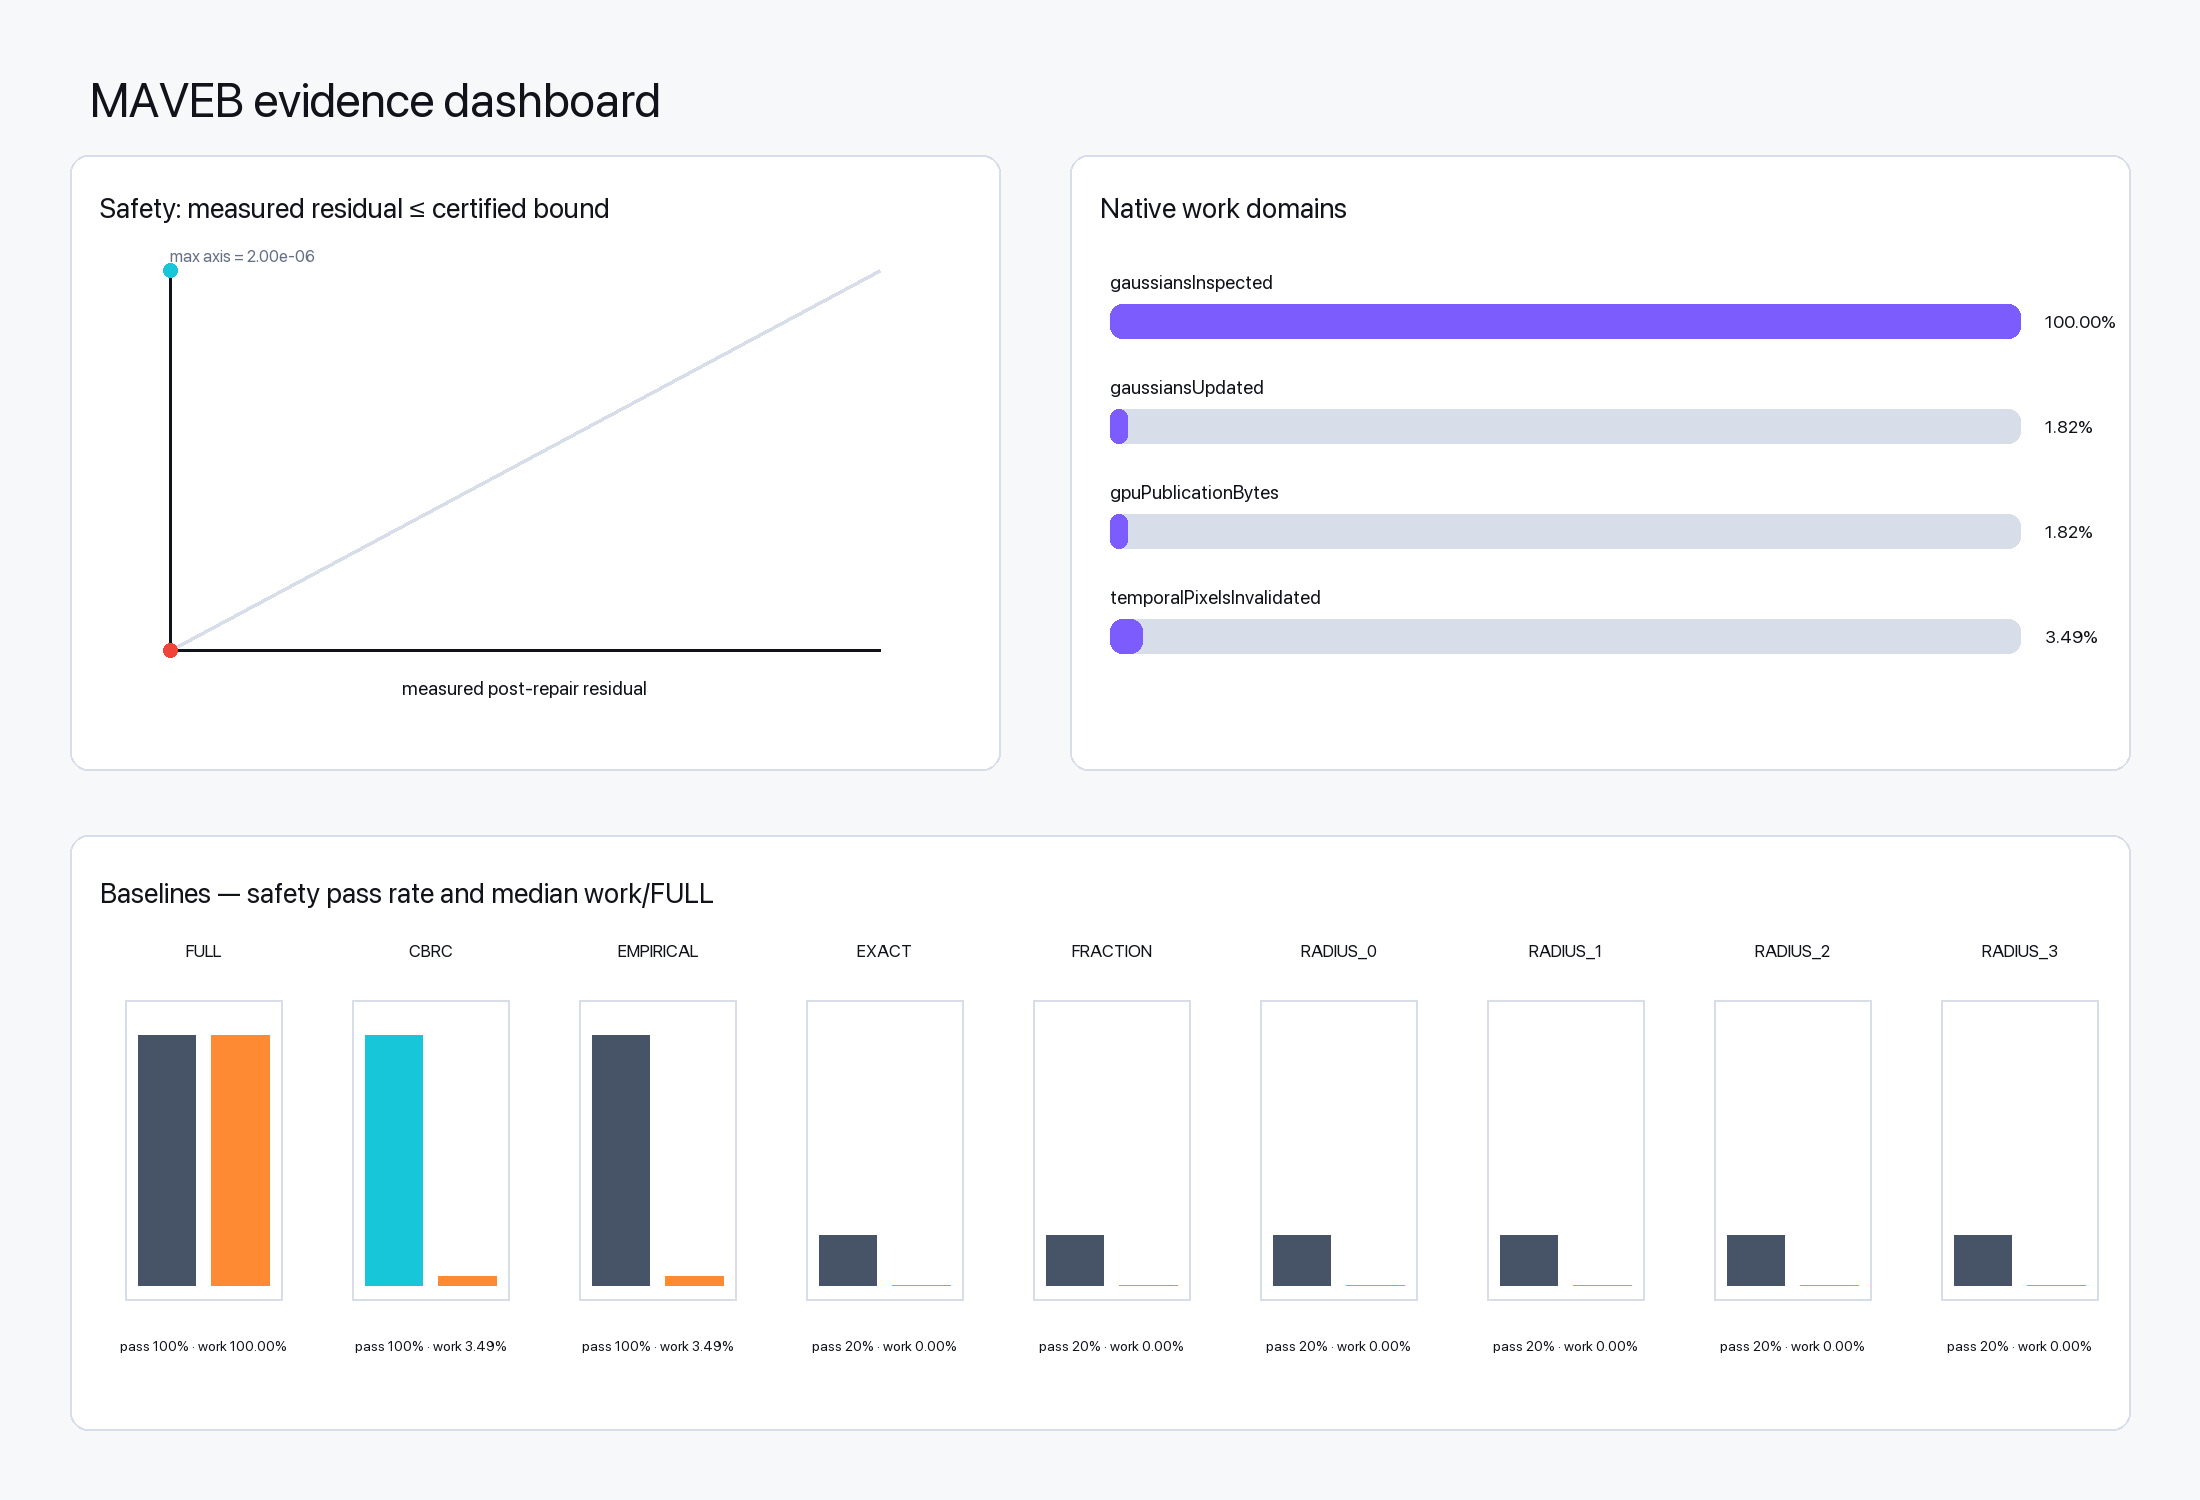
\includegraphics[width=\textwidth]{figures/trained_3dgs_evidence_dashboard.png}
\caption{Representative evidence dashboard exposing the safety check, native work domains, and baseline behavior for a trained-3DGS case.}
\end{figure}

\section{Residual-sensitive evidence chronology}
The broad 1,275-case campaign reproduces the independently generated full-after raster exactly at audited 8-bit precision, so it cannot test whether a non-zero local residual can still be safe. The residual-sensitive experiments are frozen separately.

\begin{table}[h]
\centering
\caption{Residual-sensitive sequence retained in the final claim.}
\begin{tabular}{p{0.15\textwidth}p{0.24\textwidth}p{0.52\textwidth}}
\toprule
Stage & Population & Result \\
\midrule
v4 diagnostic & 4 scenes, 512 cases & Every non-zero-residual case falls back to \textsc{Full}; this exposes the magnitude-insensitive display certificate as the bottleneck. \\
v5 mechanism & 4 scenes, 768 cases & The opacity-only delta-sensitive certificate yields 142 certified non-zero local cases and 29 tolerance crossovers; the unchanged translation control yields zero. \\
v6 confirmation & 20 scenes, 3,840 pooled parameter cases & Non-zero opacity locality and tolerance crossover occur in all 20 scenes. The scene-level opacity-minus-translation difference is 0.477 with dataset-stratified bootstrap 95\% interval [0.432, 0.517]. \\
\bottomrule
\end{tabular}
\end{table}

% Supplementary derivation for Proposition 1
% Separate from the main paper page budget.

\section*{Supplement: Gaussian finite-edit display bound}

For one protected pixel, let $U$ be the unchanged ordered Gaussian support and
$E$ the complete edited support. Effective per-splat alpha is assumed to be
post-clamp/post-cutoff and to satisfy $\alpha_i\in[0,1]$. Per-channel emitted
color after spherical-harmonic evaluation is bounded to an interval of width
$C_{\mathrm{color}}$.

For edited support $E$, define
\[
A(E)=1-\prod_{i\in E}(1-\alpha_i).
\]
This is the maximum fraction of final transmittance whose contribution can be
replaced, attenuated, or revealed through the edited splats. Since any channel
value differs by at most $C_{\mathrm{color}}$,
\[
\|R(U\cup E)-R(U)\|_\infty \le C_{\mathrm{color}}A(E).
\]

For before/after edited sets $E_0,E_1$, insert the common unchanged state $U$
and apply the triangle inequality:
\[
\begin{aligned}
\|R(U\cup E_0)-R(U\cup E_1)\|_\infty
&\le \|R(U\cup E_0)-R(U)\|_\infty\\
&\quad+\|R(U)-R(U\cup E_1)\|_\infty\\
&\le C_{\mathrm{color}}\left(A(E_0)+A(E_1)\right).
\end{aligned}
\]
The output channel itself cannot change by more than its admissible interval
width, hence
\[
\|R(U\cup E_0)-R(U\cup E_1)\|_\infty
\le C_{\mathrm{color}}\min\{1,A(E_0)+A(E_1)\}.
\]

Insertion and deletion are obtained by taking one edited set to be empty.
Depth-order changes involving edited splats are included because the edited set
must contain every Gaussian whose projected opacity, color, or order relation
can change. Renderer behavior outside these bounded assumptions is not softened
into the certificate; it becomes an exact dependency or triggers FULL fallback.
The image-space certificate is the maximum of the pixel bound over the declared
protected support.


\section{Claim boundaries}
The calibrated-work result is not a wall-clock speedup claim. Selected-to-\textsc{Full} raster equality measures revision fidelity in the evaluated representation and camera, not reconstruction quality against source photographs. The planner does not claim globally minimum-work cones. The 3,840 v6 parameter cases are pooled evidence; scene-level, dataset-stratified inference is the statistical unit. The opacity-only refinement is valid only under the paired-record invariants stated in the derivation, and unsupported cases fail closed.

\section{Ethics Statement}
N/A. This work reports software, rendering, and reconstruction experiments and does not recruit human participants or collect personal data from participants. Evaluation uses public research datasets and pretrained research assets under their upstream terms; the repository does not redistribute the upstream datasets.

\section{Generative AI Use Disclosure}
OpenAI ChatGPT was used as an assistive tool for literature-search support, software and scripting assistance, debugging, experimental planning, visualization and manuscript tooling, and drafting or language editing. Reported measurements and frozen evidence were produced by the project software and experimental artifacts. The author reviewed the final technical text and remains responsible for the code, citations, analysis, claims, conclusions, and final manuscript.

\end{document}
